\documentclass[10pt,a4paper]{article}

\usepackage{marktwo}
\usepackage{graphicx}

\begin{document}

\makemathtitle
    {The Chladni Plate}
    {A brief introduction to some continuum mechanics and the chladni plate experiment}
    {Vivek Kalita}
    {Department of Physics, IISER Mohali}
    {10 November 2026}

\tableofcontents

\section{Some Basics}

\subsection{Strain}
Consider a continuous body occupying a region of three-dimensional
space. Every material point in the body is specified by its position
vector

\[
\mathbf{r} =
\begin{pmatrix}
x\\
y\\
z
\end{pmatrix}.
\]

A deformation of the body can be described mathematically as a
mapping in which every material point is assigned a new position.
We write this mapping as

\[
\mathbf{r}\longmapsto
\mathbf{r}+\mathbf{u}(\mathbf{r})
\]
\begin{figure}[H]
    \centering
    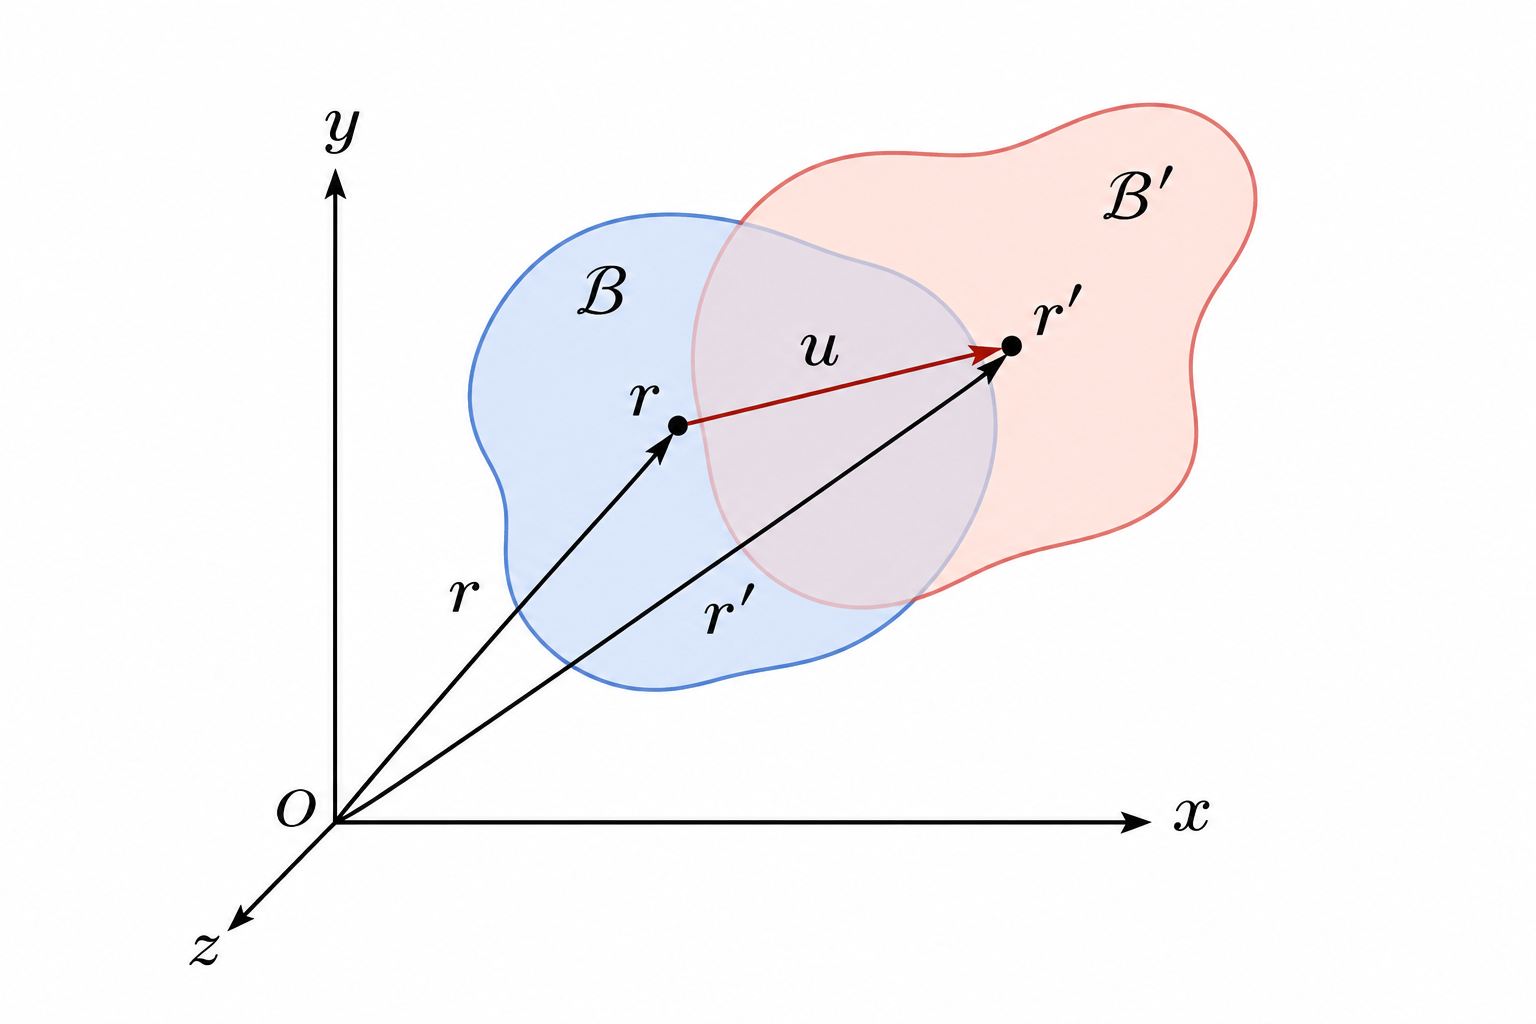
\includegraphics[width=0.55\textwidth]{chladni_plate_images/Continuum Deformation Mapping Diagram.png}
    \caption{Deformation of a continous body}
\end{figure}
where \(\mathbf{u}(\mathbf{r})\) is the displacement vector field,
given by

\[
\mathbf{u}(\mathbf{r}) =
\begin{pmatrix}
u_x(x,y,z)\\
u_y(x,y,z)\\
u_z(x,y,z)
\end{pmatrix}.
\]

\begin{enumerate}
    \item Now consider an infinitesimal rectangular element of a continuous
medium with dimensions \(dx\), \(dy\) and \(dz\). 
\begin{figure}[H]
    \centering
    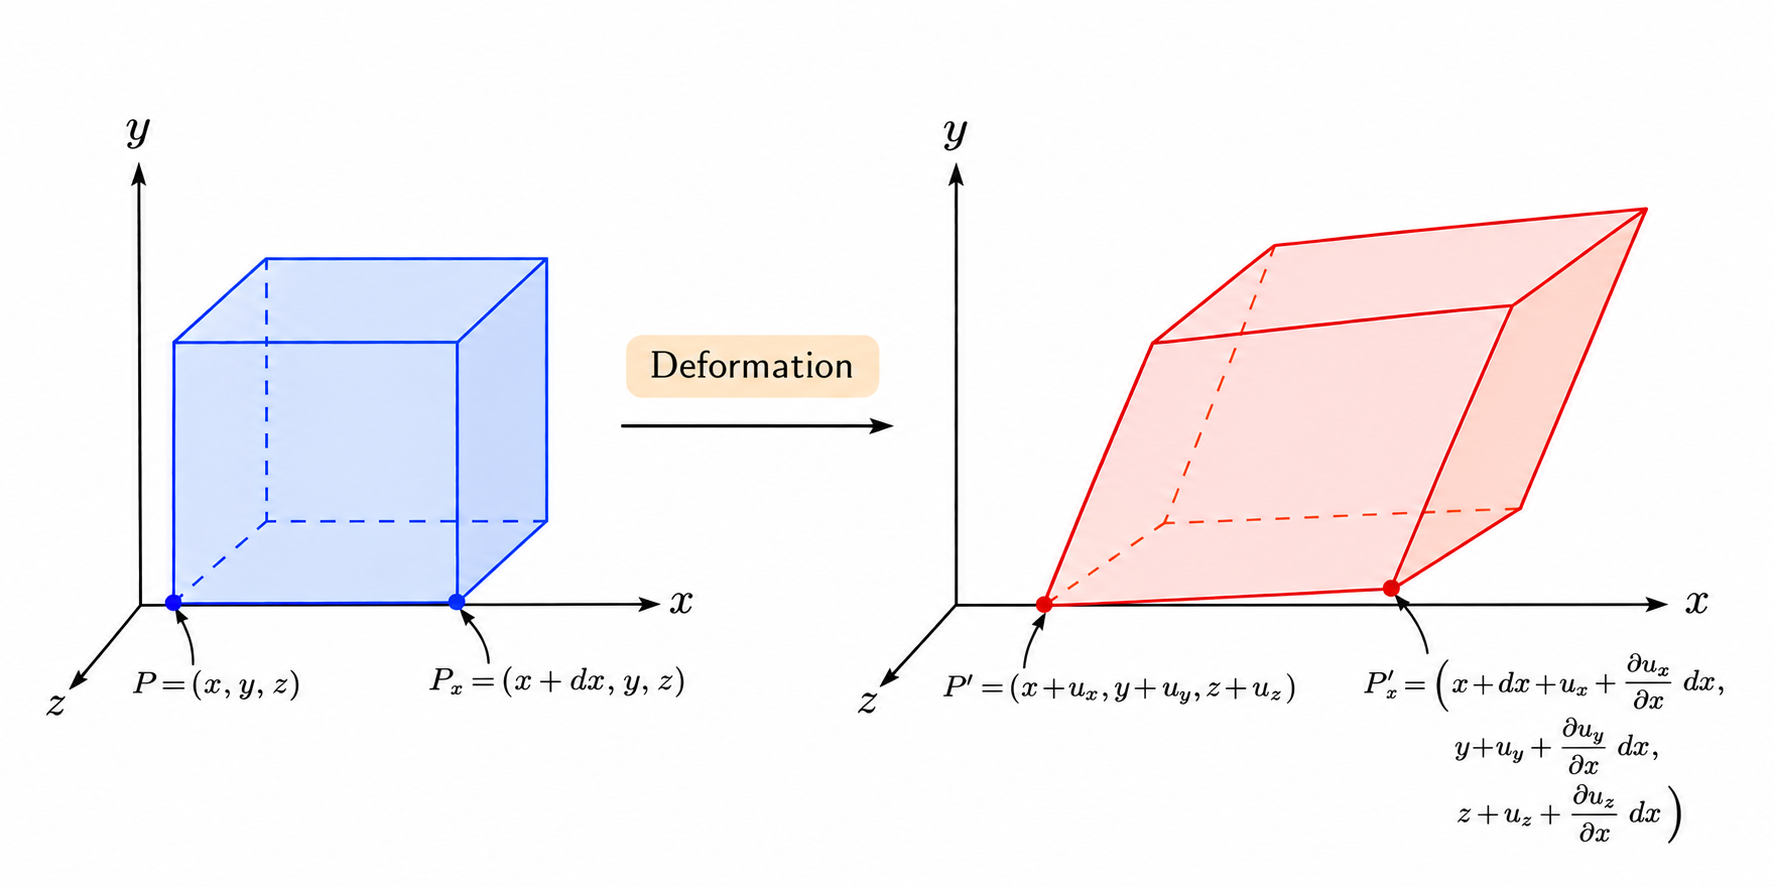
\includegraphics[width=0.8\textwidth]{chladni_plate_images/deformation.png}
    \caption{Deformations of a very small cuboid}
\end{figure}
Let one of its
vertices be located at \(P=(x,y,z).\) The three neighbouring vertices along the coordinate directions
are initially located at

\[
P_x=(x+dx,y,z), \qquad
P_y=(x,y+dy,z), \qquad
P_z=(x,y,z+dz).
\]

Under a deformation, every material point is displaced according
to the displacement field

\[
\mathbf{u}(x,y,z)
=
\left(
u_x(x,y,z),\,
u_y(x,y,z),\,
u_z(x,y,z)
\right).
\]

Consequently, the point \(P\) is mapped to

\[
P'=
\left(
x+u_x(x,y,z),\,
y+u_y(x,y,z),\,
z+u_z(x,y,z)
\right).
\]

Similarly, the neighbouring point \(P_x\) is mapped to

\[
P_x'=
\left(
x+dx+u_x(x+dx,y,z),\,
y+u_y(x+dx,y,z),\,
z+u_z(x+dx,y,z)
\right).
\]

Expanding the displacement components in a Taylor series
about \((x,y,z)\), and retaining only the first-order terms,
we obtain the change in the position of the neighbouring
point relative to \(P'\) to be:

\[
P_x'-P'
=
\left(
\left(1+\frac{\partial u_x}{\partial x}\right)dx,\,
\frac{\partial u_y}{\partial x}dx,\,
\frac{\partial u_z}{\partial x}dx
\right).
\]
In particular, the change in the length of the edge along
the \(x\)-direction, to first order, is

\[
\Delta x=
\frac{\partial u_x}{\partial x}\,dx.
\]

\item \textcolor{red!70!black}{\textsf{Strain}} is defined as the fractional change in length,
the normal strain along the \(x\)-direction is

\[
\epsilon_{xx}
=
\frac{\Delta x}{dx}
=
\frac{\partial u_x}{\partial x}.
\]

Following the same procedure for the edges along the
\(y\) and \(z\) directions, we obtain

\[
\epsilon_{yy}=\frac{\partial u_y}{\partial y},
\qquad
\epsilon_{zz}=\frac{\partial u_z}{\partial z}.
\]
\item From the previous calculations, we know that the change
in height of the edge parallel to the \(x\)-axis is

\[
\Delta y = \frac{\partial u_y}{\partial x}\,dx.
\]

Therefore, for small deformations,

\[
\alpha \approx \tan\alpha
= \frac{\Delta y}{dx}
= \frac{\partial u_y}{\partial x}.
\]

Similarly, we can obtain

\[
\beta \approx \tan\beta
= \frac{\partial u_x}{\partial y}.
\]

\begin{figure}[H]
    \centering
    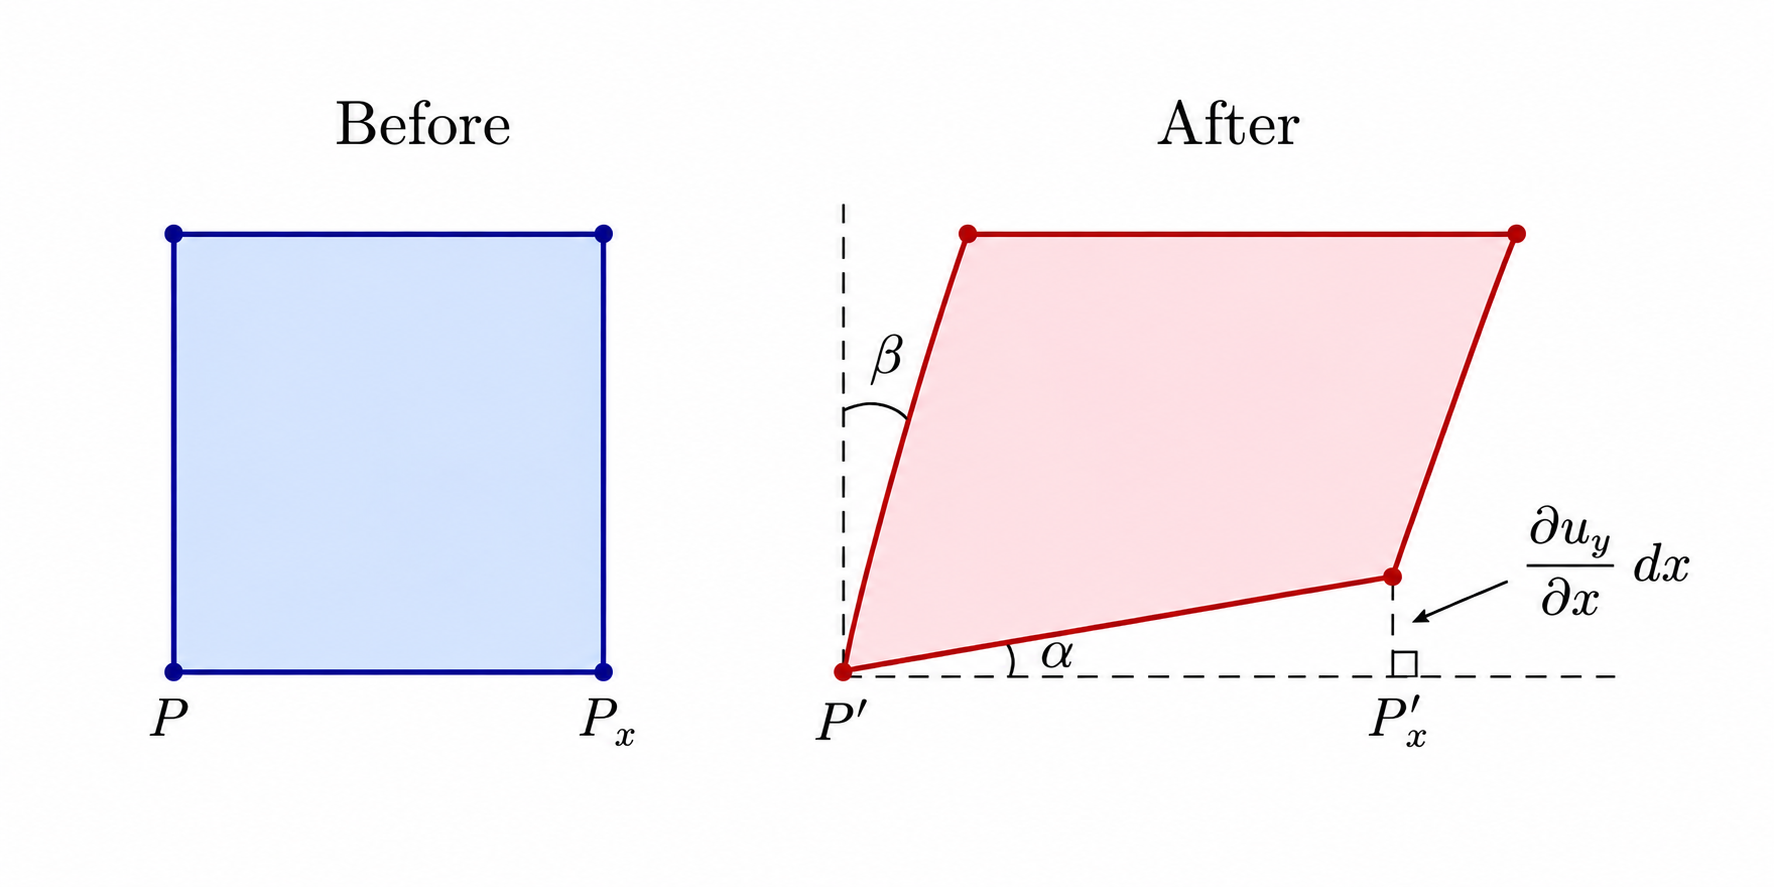
\includegraphics[width=0.7\textwidth]{chladni_plate_images/shear_stress.png}
    \caption{The shear strain}
\end{figure}
The total change in the right angle between the two edges is
given by the sum of these two angles. Hence,

\[
\gamma_{xy} = \alpha+\beta
= \frac{\partial u_y}{\partial x}
+ \frac{\partial u_x}{\partial y}.
\]

This quantity is called the \textcolor{red!70!black}{\textsf{engineering shear strain.}}

\item Therefore, the engineering shear strains are

\[
\gamma_{xy}
=
\frac{\partial u_y}{\partial x}
+
\frac{\partial u_x}{\partial y}
\quad
\gamma_{yx}
=
\frac{\partial u_x}{\partial y}
+
\frac{\partial u_y}{\partial x}.
\]

By convention, the components of the infinitesimal strain
tensor are defined as half the engineering shear strain.
Thus,

\[
\epsilon_{xy}=\epsilon_{yx}
=
\frac{1}{2}
\left(
\frac{\partial u_y}{\partial x}
+
\frac{\partial u_x}{\partial y}
\right).
\]
\end{enumerate}

\begin{definition}[Strain Tensor]
The strain tensor is a second-order symmetric tensor that
describes the deformation of a continuous body. It is given by

\[
\boldsymbol{\epsilon}
=
\begin{pmatrix}
\epsilon_{xx} & \epsilon_{xy} & \epsilon_{xz}\\
\epsilon_{yx} & \epsilon_{yy} & \epsilon_{yz}\\
\epsilon_{zx} & \epsilon_{zy} & \epsilon_{zz}
\end{pmatrix}.
\]

The diagonal components represent normal strains, given by

\[
\epsilon_{xx}=\frac{\partial u_x}{\partial x}
\quad
\epsilon_{yy}=\frac{\partial u_y}{\partial y}
\quad
\epsilon_{zz}=\frac{\partial u_z}{\partial z}.
\]

The off-diagonal components represent shear strains:

\[
\epsilon_{xy}=\epsilon_{yx}
=\frac{1}{2}\left(
\frac{\partial u_x}{\partial y}
+\frac{\partial u_y}{\partial x}
\right), \quad
\epsilon_{yz}=\epsilon_{zy}
=\frac{1}{2}\left(
\frac{\partial u_y}{\partial z}
+\frac{\partial u_z}{\partial y}
\right),
\quad
\epsilon_{xz}=\epsilon_{zx}
=\frac{1}{2}\left(
\frac{\partial u_x}{\partial z}
+\frac{\partial u_z}{\partial x}
\right).
\]
\end{definition}

\subsection{Strain}
\begin{assumption}
We consider a material satisfying the following assumptions:

\begin{enumerate}[label=\textsf{\textcolor{red!70!black}{A\arabic*.}}]

    \item \textsf{\textcolor{blue}{Homogeneous.}}
    Its material properties are identical throughout.

    \item \textsf{\textcolor{blue}{Isotropic.}}
    Its material properties are identical in every direction.

    \item \textsf{\textcolor{blue}{Linearly Elastic.}}
    The stress is linearly related to the strain for sufficiently
    small deformations, allowing us to use the principle of
    superposition.

\end{enumerate}
\end{assumption}

\textcolor{red!70!black}{\textsf{Young's modulus}} is defined as the ratio of longitudinal
stress to longitudinal strain, i.e.

\[
E=\frac{\text{Longitudinal Stress}}{\text{Longitudinal Strain}}.
\]

When a block is stretched along a particular direction, say the
\(x\)-direction, it contracts along the two perpendicular
directions. 

Since the material is isotropic, its elastic response
is independent of the direction of loading. The Poisson's ratio (which is defined as the negative ratio of transverse strain to longitudinal strain) is thereofore constant. For a uniaxial stress in the \(x\)-direction, we have

\[
\nu=-\frac{\epsilon_{yy}}{\epsilon_{xx}}
\quad
\nu=-\frac{\epsilon_{zz}}{\epsilon_{xx}}.
\]

Similarly, for uniaxial loading along the \(y\) and \(z\) directions,
the corresponding relations are

\[
\nu=-\frac{\epsilon_{xx}}{\epsilon_{yy}}
=-\frac{\epsilon_{zz}}{\epsilon_{yy}}
\quad
\nu=-\frac{\epsilon_{xx}}{\epsilon_{zz}}
=-\frac{\epsilon_{yy}}{\epsilon_{zz}}.
\]

\begin{enumerate}
    \item \textcolor{red!70!black}{Normal Stress} Consequently, when a uniaxial stress \(\sigma\) is applied along
the \(x\)-direction, we obtain

\[
\epsilon_{xx}=\frac{\sigma}{E}
\quad
\epsilon_{yy}=-\frac{\nu\sigma}{E}
\quad
\epsilon_{zz}=-\frac{\nu\sigma}{E}.
\]

Now suppose that we apply three normal stresses simultaneously,
namely \(\sigma_{xx}\), \(\sigma_{yy}\) and \(\sigma_{zz}\).
Since the material is linearly elastic, we can use the
principle of superposition.

Consider the strain along the \(x\)-direction.
    The individual contributions are:

    \begin{enumerate}

        \item The stress \(\sigma_{xx}\) produces a longitudinal
        strain

        \[
        \epsilon_{xx}^{(1)}=\frac{\sigma_{xx}}{E}.
        \]

        \item The stress \(\sigma_{yy}\) produces a transverse
        strain along the \(x\)-direction

        \[
        \epsilon_{xx}^{(2)}=-\frac{\nu\sigma_{yy}}{E}.
        \]

        \item Similarly, the stress \(\sigma_{zz}\) produces
        a transverse strain along the \(x\)-direction

        \[
        \epsilon_{xx}^{(3)}=-\frac{\nu\sigma_{zz}}{E}.
        \]

    \end{enumerate}

Adding all the contributions, we obtain

\[
\epsilon_{xx}
=
\epsilon_{xx}^{(1)}
+\epsilon_{xx}^{(2)}
+\epsilon_{xx}^{(3)}
=
\frac{1}{E}
\left[
\sigma_{xx}-\nu(\sigma_{yy}+\sigma_{zz})
\right].
\]

By symmetry, the corresponding relations along the \(y\) and
\(z\) directions are

\[
\epsilon_{yy}
=
\frac{1}{E}
\left[
\sigma_{yy}-\nu(\sigma_{xx}+\sigma_{zz})
\right],
\quad 
\epsilon_{zz}
=
\frac{1}{E}
\left[
\sigma_{zz}-\nu(\sigma_{xx}+\sigma_{yy})
\right].
\]
\item \textsf{\textcolor{red!70!black}{Shear stress}} Hooke's law for shear is
\[
\tau = G\gamma,
\]
where \textsf{\textcolor{blue!70!black}{engineering shear strain}} is denoted by \(\gamma\), and \(G\) is the \textsf{\textcolor{blue!70!black}{shear modulus}}. We also have
\[
G = \frac{E}{2(1+\nu)}.
\]
\end{enumerate}

\begin{theorem}[Tensor form of Hooke's law]
For an \textcolor{red!70!black}{\textnormal{\textsf{isotropic, linearly elastic body}}}, the stress-strain
relation in tensor form is given by
\[
\boldsymbol{\sigma}
=
\lambda\,\operatorname{tr}(\boldsymbol{\epsilon})I
+2G\boldsymbol{\epsilon},
\]
where
\[
\lambda=\frac{E\nu}{(1+\nu)(1-2\nu)}.
\]
Here, \(E\) is Young's modulus, \(\nu\) is Poisson's ratio,
\(G\) is the shear modulus, and \(I\) is the identity tensor.
\end{theorem}

\subsection{Newton's laws and the Navier--Cauchy equation}
\begin{enumerate}

    \item Consider a small rectangular element of a continuous body
    with dimensions \(dx\), \(dy\) and \(dz\). Its volume and mass
    are \(dV = dx\,dy\,dz\) and \(dm = \rho\,dV\), respectively.

    The element experiences two kinds of forces:

    \begin{enumerate}

        \item \textsf{\textcolor{red!70!black}{Surface forces.}}
        These are the forces exerted by the surrounding material
        on the faces of the element. They arise due to the
        stress tensor, which is given by
        \[
        \boldsymbol{\sigma} =
        \begin{pmatrix}
        \sigma_{xx} & \sigma_{xy} & \sigma_{xz}\\
        \sigma_{yx} & \sigma_{yy} & \sigma_{yz}\\
        \sigma_{zx} & \sigma_{zy} & \sigma_{zz}
        \end{pmatrix}.
        \]

        Consider first the two faces whose normals point along
        the \(x\)-direction. The face at position \(x\) experiences
        an \(x\)-directed force
        \[
        F_x^{(-)}=-\sigma_{xx}(x,y,z)\,dy\,dz,
        \]
        whereas the opposite face at \(x+dx\) experiences
        \[
        F_x^{(+)}=\sigma_{xx}(x+dx,y,z)\,dy\,dz.
        \]

        Adding these contributions and using a first-order
        Taylor expansion, we obtain
        \[
        F_x^{(1)}
        =\frac{\partial \sigma_{xx}}{\partial x}\,dV.
        \]

        \begin{figure}[H]
            \centering
            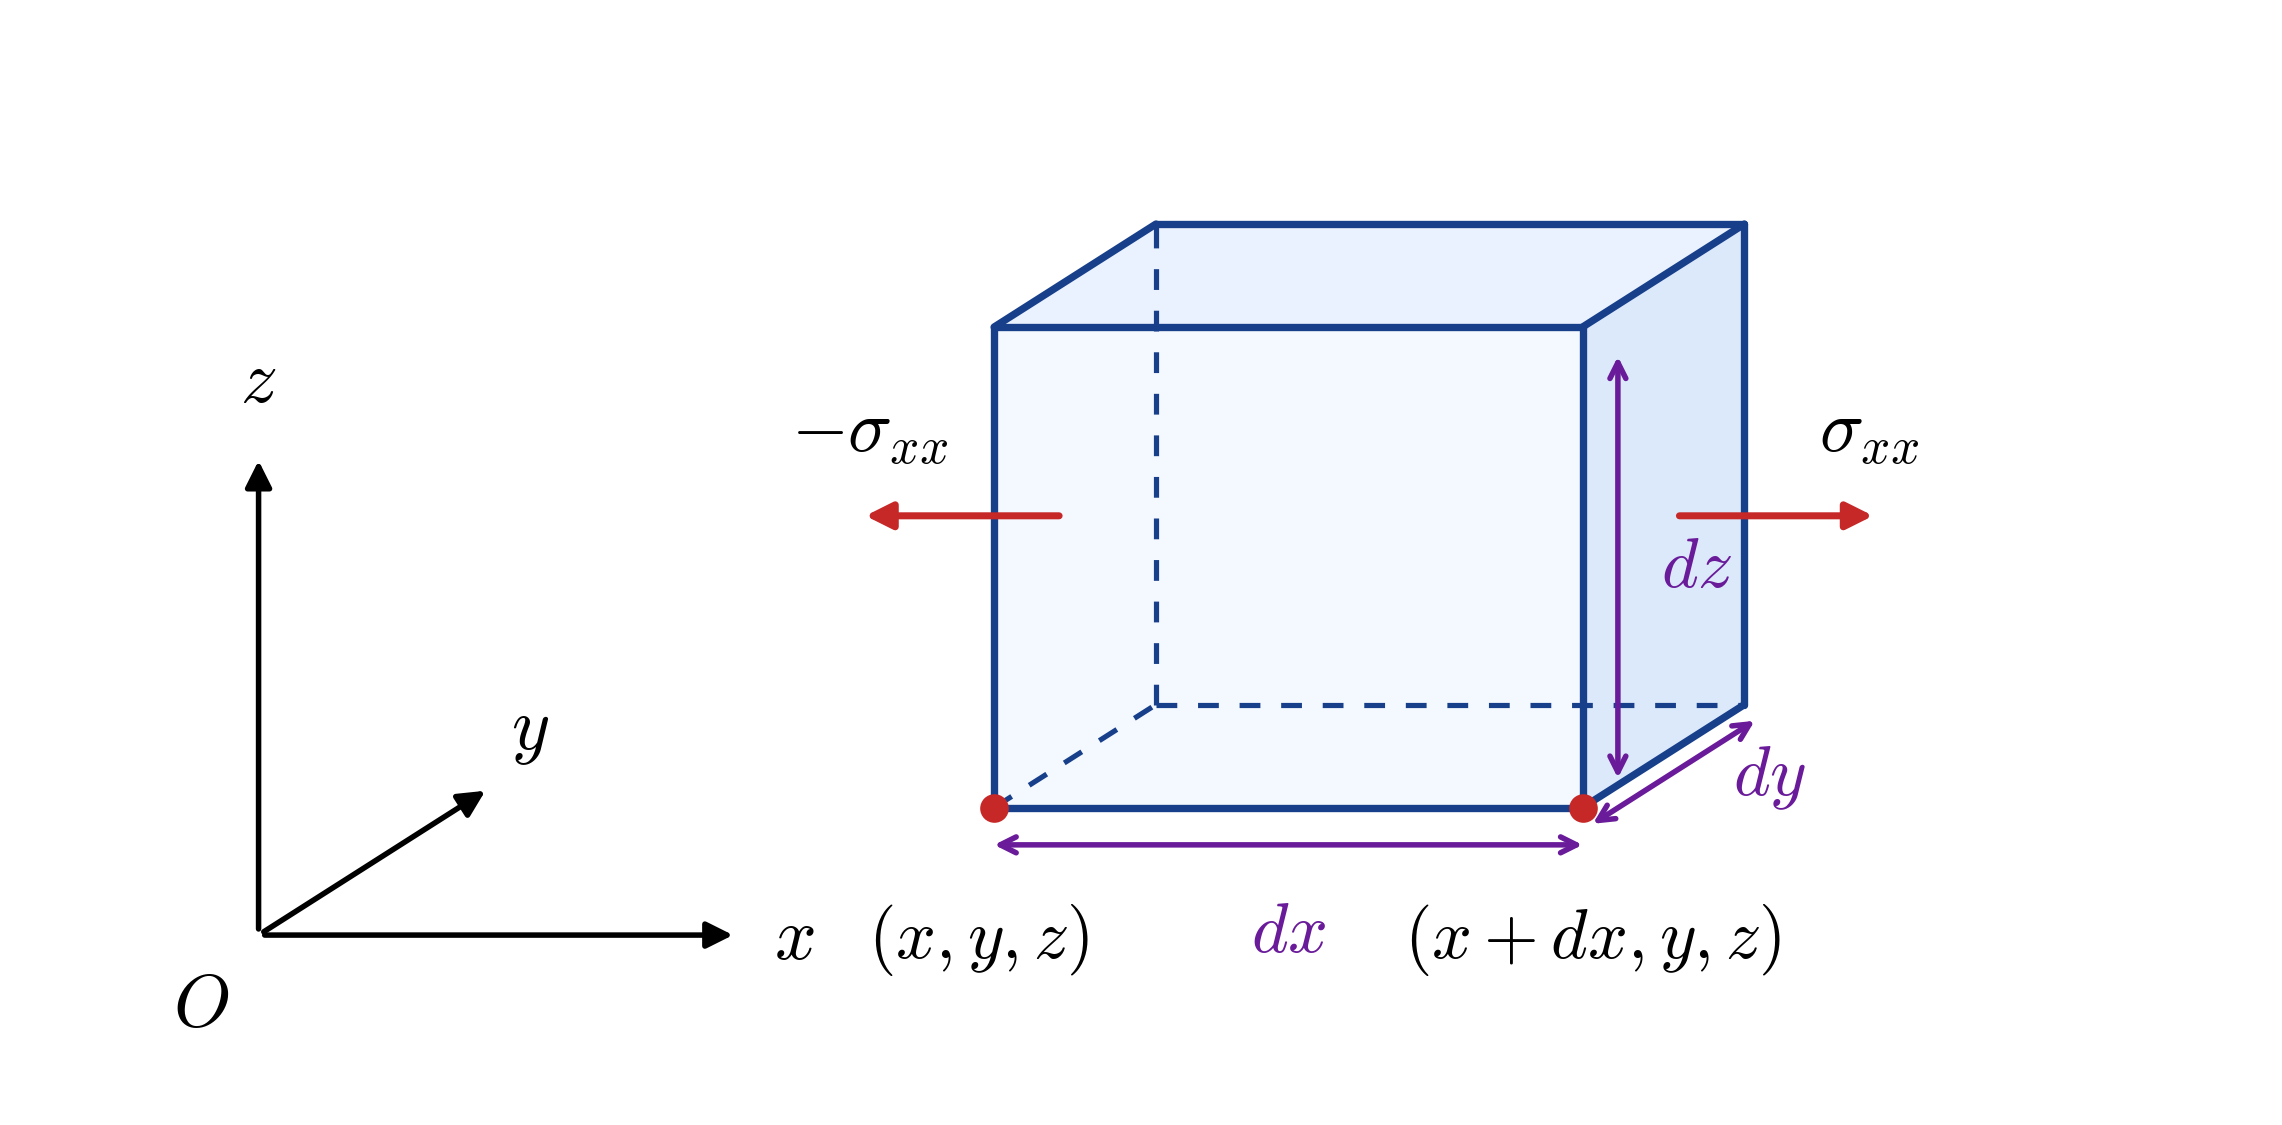
\includegraphics[width=0.75\textwidth]{chladni_plate_images/stressonbody.png}
            \caption{Force due to surrounding material}
        \end{figure}
        Similarly, the contributions from the two pairs of faces
        normal to the \(y\)- and \(z\)-directions are
        \[
        F_x^{(2)}
        =\frac{\partial \sigma_{xy}}{\partial y}\,dV,
        \qquad
        F_x^{(3)}
        =\frac{\partial \sigma_{xz}}{\partial z}\,dV.
        \]

        Thus, the total surface force along the \(x\)-direction is
        \[
        F_x^{\mathrm{surface}}
        =
        \left(
        \frac{\partial \sigma_{xx}}{\partial x}
        +\frac{\partial \sigma_{xy}}{\partial y}
        +\frac{\partial \sigma_{xz}}{\partial z}
        \right)dV.
        \]

        Repeating the same procedure along the \(y\)- and
        \(z\)-directions, we obtain the total surface force
        in vector form:
        \[
        \mathbf{F}_{\mathrm{surface}}
        =
        (\nabla\cdot\boldsymbol{\sigma})\,dV,
        \]
        where
       \[
\nabla\cdot\boldsymbol{\sigma}
=
\begin{pmatrix}
\dfrac{\partial}{\partial x} &
\dfrac{\partial}{\partial y} &
\dfrac{\partial}{\partial z}
\end{pmatrix}
\begin{pmatrix}
\sigma_{xx} & \sigma_{xy} & \sigma_{xz}\\
\sigma_{yx} & \sigma_{yy} & \sigma_{yz}\\
\sigma_{zx} & \sigma_{zy} & \sigma_{zz}
\end{pmatrix}.
\]
        \item \textsf{\textcolor{red!70!black}{Body forces.}}
        These are forces that act throughout the volume of the
        element, such as gravitational forces. Let the body force
        per unit volume be represented by
        \[
        \mathbf{f} =
        \begin{pmatrix}
        f_x\\
        f_y\\
        f_z
        \end{pmatrix}.
        \]
        Therefore, the total body force acting on the element is
        \[
        \mathbf{F}_{\mathrm{body}}=\mathbf{f}\,dV.
        \]

    \end{enumerate}

    \item The net force acting on the infinitesimal element is therefore
\[
\mathbf{F}_{\mathrm{net}}
=
\left(
\nabla\cdot\boldsymbol{\sigma}+\mathbf{f}
\right)dV.
\]

Applying Newton's second law, we have
\[
\rho\mathbf{a}
=
\nabla\cdot\boldsymbol{\sigma}+\mathbf{f}.
\]
\end{enumerate}

\begin{theorem}[Newton's law for a continuum]
According to Newton's second law, the equation of motion for a
continuum is given by
\[
\rho\mathbf{a}
=
\nabla\cdot\boldsymbol{\sigma}
+\mathbf{f},
\]
where \(\rho\) is the mass density, \(\mathbf{a}\) is the
acceleration vector, \(\boldsymbol{\sigma}\) is the stress tensor,
and \(\mathbf{f}\) is the external body force per unit volume.
\end{theorem}

\section{The Chladni Plate}
\begin{enumerate}

    \item Consider a thin plate of thickness \(h\), occupying the
    region \(-h/2\leq z\leq h/2\). Initially, its middle surface
    lies in the \(xy\)-plane (so that any point on the middle surface is \(\mathbf{r}(x,y)=(x,y,0)\)). 

    Assume that after deformation, the middle surface is displaced in the
    \(z\)-direction by an amount \(w(x,y,t)\). Its position vector
    therefore becomes
    \(\mathbf{r}'(x,y,t)=(x,y,w(x,y,t))\).

    The normal vector to the deformed middle surface (assuming small slopes, that is,
    \(\lvert w_x\rvert,\lvert w_y\rvert\ll 1\)) is given by
    \[
    \mathbf{n}=
    \begin{pmatrix}
    -w_x\\
    -w_y\\
    1
    \end{pmatrix}.
    \]
\item According to the \textsf{\textcolor{red!70!black}{Kirchhoff--Love hypothesis}} (for thin plates), any point initially lying along the normal to the middle surface moves along the normal to the deformed middle surface. Furthermore, the normal remains straight and its length remains unchanged.

    Thus, a point initially located at \(\mathbf{r}=(x,y,z)\) is transported to the position
    \[
    \mathbf{r}'= (x,y,w)+z(-w_x,-w_y,1)= (x-zw_x,\ y-zw_y,\ w+z).
    \]
    
\begin{figure}[H]
    \centering
    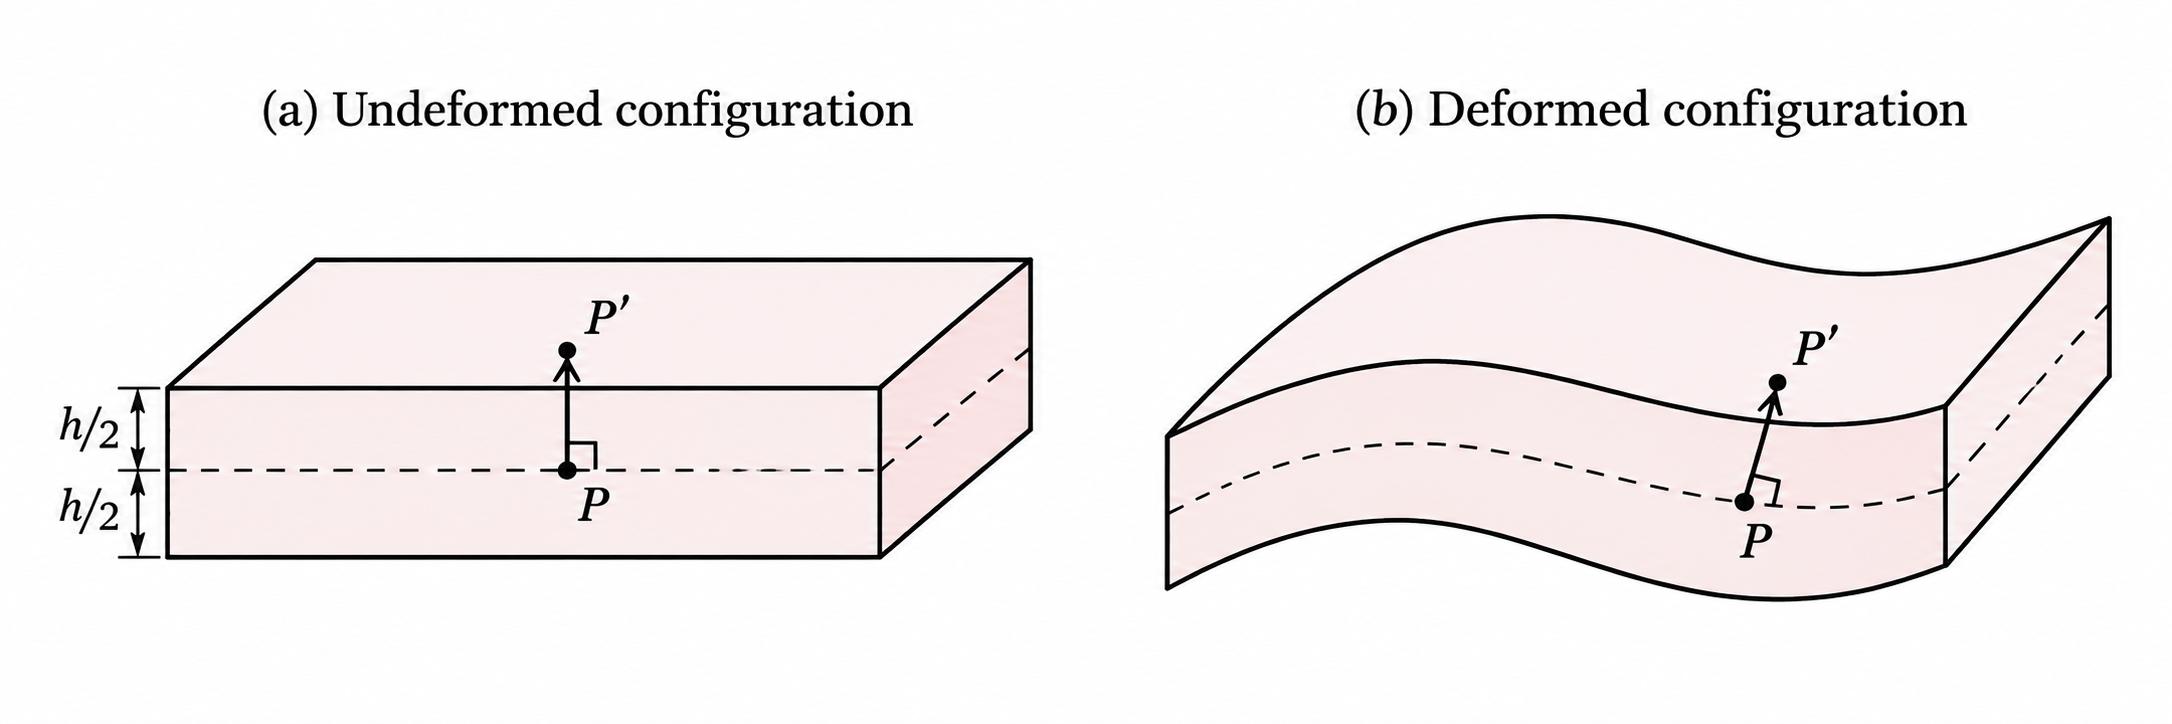
\includegraphics[width=0.75\textwidth]{chladni_plate_images/kirchoff-love.png}
    \caption{Illustration of the Kirchhoff-Love law (this actually is prety intuitive)}
\end{figure}
\item The displacement field is thus given by (note that \(w=w(x,y,t)\)):
\[
\mathbf{u}
=
\begin{pmatrix}
-zw_x , -zw_y , w
\end{pmatrix},
\]

The strain tensor therefore is:
\[
\boldsymbol{\epsilon}
=
-z
\begin{pmatrix}
w_{xx} & w_{xy} & 0\\
w_{xy} & w_{yy} & 0\\
0 & 0 & 0
\end{pmatrix}.
\]
\item The equations of motion for the plate are given by the
three components of Newton's law:
\[
\begin{aligned}
\frac{\partial\sigma_{xx}}{\partial x}
+\frac{\partial\sigma_{xy}}{\partial y}
+\frac{\partial\sigma_{xz}}{\partial z}
&=\rho\frac{\partial^2u_x}{\partial t^2}
=-\rho z w_{xtt},\\[8pt]
\frac{\partial\sigma_{xy}}{\partial x}
+\frac{\partial\sigma_{yy}}{\partial y}
+\frac{\partial\sigma_{yz}}{\partial z}
&=\rho\frac{\partial^2u_y}{\partial t^2}
=-\rho z w_{ytt},\\[8pt]
\frac{\partial\sigma_{xz}}{\partial x}
+\frac{\partial\sigma_{yz}}{\partial y}
+\frac{\partial\sigma_{zz}}{\partial z}
&=\rho\frac{\partial^2u_z}{\partial t^2}
=\rho w_{tt}.
\end{aligned}
\]
\end{enumerate}

\end{document}